\chapter{MixVRTの実装}\label{cha:Implementation}
本章では、\toolName の実装について説明する。
\toolName のシステム構成を、図\ref{fig:System}に示す。
\begin{figure}[tp]
    \begin{center}
        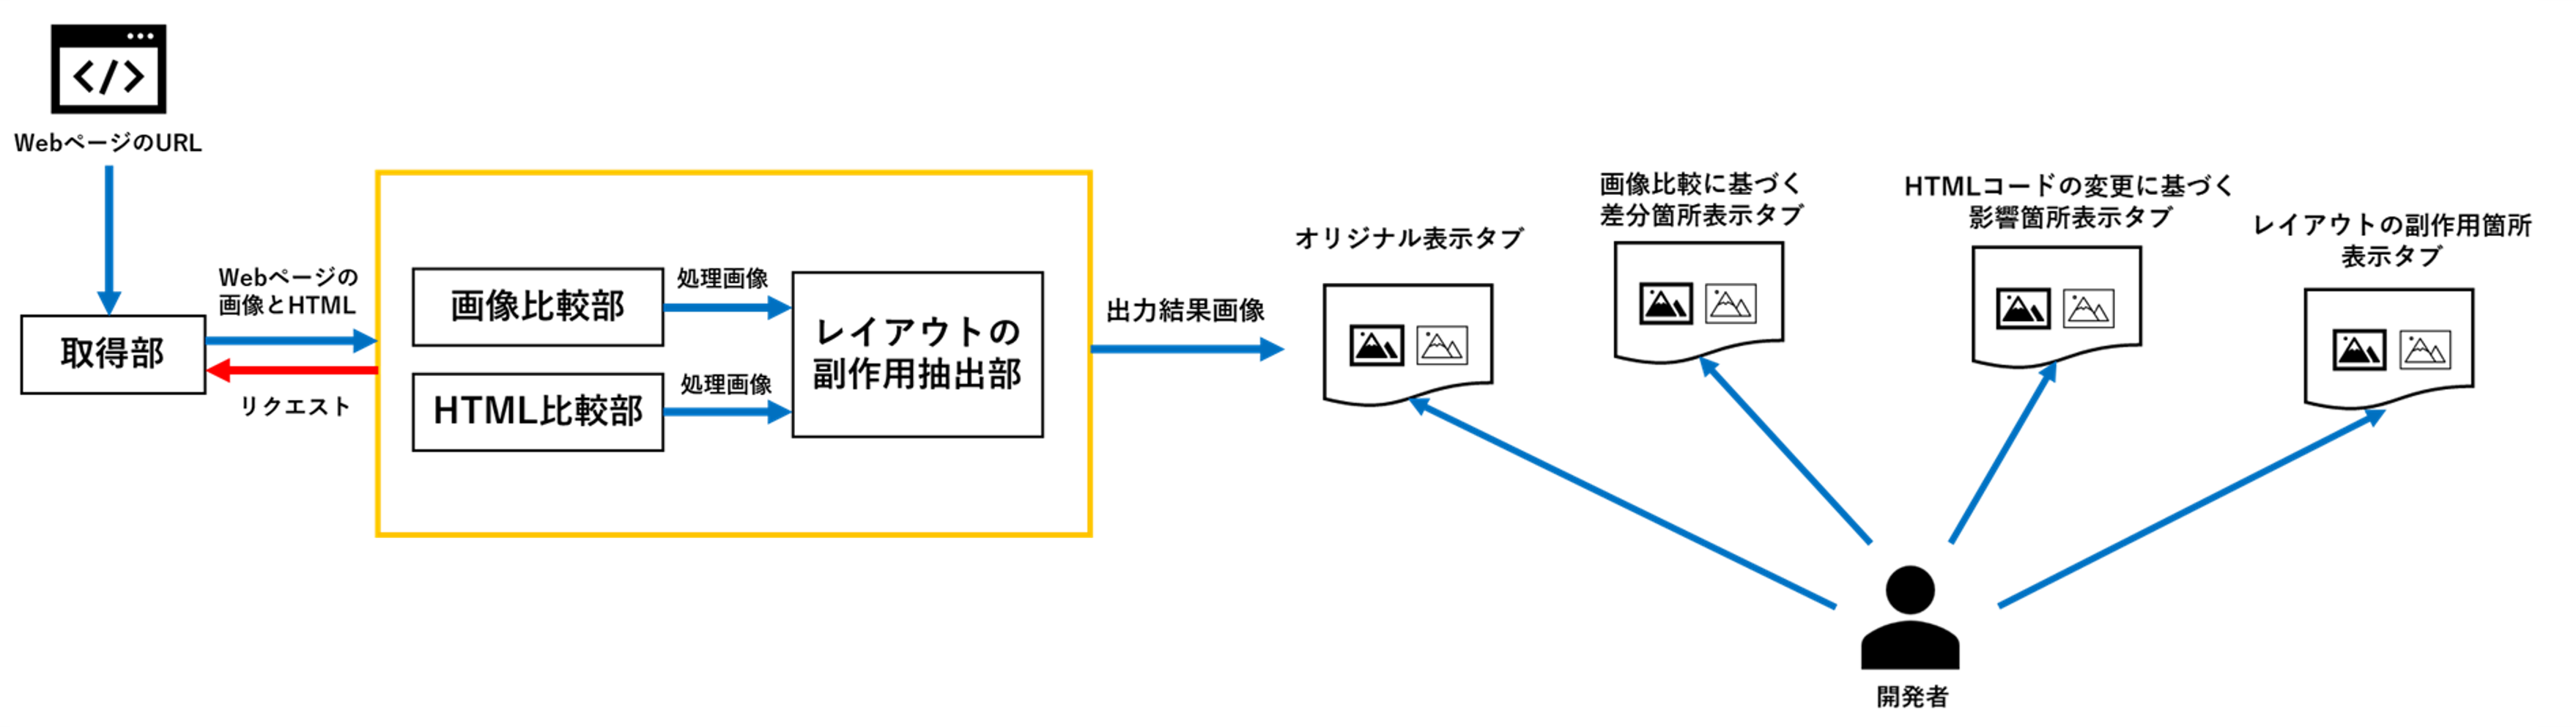
\includegraphics[width=1.0\columnwidth]{image/4_System.png}
        \caption{\toolName のシステム構成}
        \label{fig:System}
    \end{center}
\end{figure}
% 私の開発したツールは、まずユーザーがWebページのURLを入力します。
% このURLを受け取ると、ツールは該当するWebページから画像を取得し、
% これらの画像に対して特定の処理を行います。処理された画像は"static/images"ディレクトリに保存されます。
% そして、Flaskがローカルサーバを提供し、
% "templates"フォルダにあるHTMLファイルが"static/images"ディレクトリを参照できるようになっています。
% この仕組みにより、ユーザーはローカルに立てられたFlaskサーバを通じて、
% Webページ上で生成された画像を確認することができます。
本研究では、\toolName の試作にあたり、以下の5つの処理部を実装する。
\begin{itemize}
    \item Webデータ取得部
    \item 画像比較部
    \item 画像差分箇所検出部
    \item HTML影響箇所抽出部
    \item HTML解析部
    \item HTML影響箇所検出部
    \item レイアウトの副作用箇所抽出部
    \item インターフェース表示部
\end{itemize}
以降、\toolName を構成する5つの処理部について説明する。
\par



\section{Webページ情報取得部}\label{sec:Web_page_information_get_section}
Webページ情報取得部は、WebページのURLを入力としてもらい、Webページの画像とHTMLコードを取得する。
Webページの画像取得には、Selenium WebDriverを用いてWebページの画像を取得する。
Seleniumスクリプトにより、\toolName の入力であるWebページのURLにアクセスし、Webページの画像を取得する。
HTMLコード取得には、Pythonライブラリの一つであるrequestsモジュールを用いて、WebページのURLからHTMLコードを取得する。


\section{画像比較に基づく差分箇所抽出部}\label{sec:Difference_extraction_section}
画像比較に基づく差分箇所抽出部は、Webページ情報取得部で取得したWebページの画像のみを用いて、画像比較を行う。
画像比較には、PythonのOpenCvを用いて比較を行う。画像比較の手順を以下に示す。
\begin{enumerate}
    \item 高解像度画像生成処理
    \item 適応的二値化処理
    \item 差分検出処理
    \item 膨張処理
    \item 輪郭検出処理
    \item バウンディングボックス描画処理
\end{enumerate}

\subsection{高解像度画像生成処理}\label{subsec:Generate_high_images}
高解像度画像の生成は、元のWebページ画像をもとに高解像度の画像を生成する。高解像度の画像はのちの輪郭検出処理の精度を向上するために必要である。
元のWebページ画像はpng画像であり、png画像をsvgファイルに変換し、さらにsvgファイルをpdfファイルに変換した後、pdfファイルをpng画像に戻す処理を行うことで、高解像度のpng画像を生成することができる。
まず、png画像をsvg画像に変換するには、Aspose.Wordsライブラリのaw.Document()とaw.DocumentBuilder()を使用して、png画像をドキュメントに挿入し、Aspose.WordsのImageSaveOptionsを使用して、画像をsvg形式で保存する。
次に、svg画像からpdf画像に変換するには、svglibとreportlabライブラリを使用して、svgファイルをpdfファイルに変換する。
最後にpdfファイルからpng画像に変換するには、pdf2imageライブラリのconvert\_from\_path関数を使用して、pdfファイルをpng画像に変換する。この際、解像度を300DPI(Dots Per Inch:1インチ当たりのドット数)に設定することで、
150DPI(Dots Per Inch)である元のWebページ画像の2倍解像度が高解像度画像を生成する。

% アンダーバー"_"は"\"でエスケープする

\subsection{適応的二値化処理}\label{subsec:Adaptive_Binarisation}
適応的二値化処理は、Webページ画像の二値化(白黒化)を行う。
Webページ画像を二値化する流れを、以下に示す。
\begin{enumerate}
    \item OpenCVのimread関数を用いて、Webページ画面画像をグレースケール画像に変換して読み込む。
\end{enumerate}


\subsection{差分検出処理}\label{subsec:difference_detection_process}


\subsection{膨張処理}\label{subsec:dilation}


\subsection{輪郭検出処理}\label{subsec:contour_detection_processing}


\subsection{バウンディングボックス描画処理}\label{subsec:Bounding box drawing process}



\section{HTMLコードの変更に基づく影響箇所抽出部}\label{sec:Affected_area_extraction}
HTMLコードの変更に基づく影響箇所抽出部は、Webページ情報取得部で取得した変更前後のWebページのHTMLコードを用いて影響箇所を特定する。
概要としては、差分ファイルを生成し、差分ファイルから枠付け処理を行った変更前後のHTMLコードを生成した後、そのHTMLコードをFlaskのテンプレートエンジンを用いてWebページを表示し、Webページ情報取得部によってそのWebページの画像を取得する。
元のWebページ画像と枠付け処理をしたWebページ画像を比較して枠のみを抽出する。
具体的には、まず、Pythonライブラリの一つであるdifflibモジュールを用いて、変更前後のHTMLコードから差分ファイルを生成する。
生成した差分ファイルは、コードの追加行には"+", 削除行には"-", 変更前後のHTMLコードにどちらにも存在しない行には"?"が先頭に付き、"?"を除いた差分ファイルを解析対象とする。
差分ファイルは、bodyタグ内とstyleタグ内を対象とする。
もし、bodyタグ内で先頭に"+"や"-"があれば、コードの追加や削除、変更があったとして、その箇所に枠付け処理を行うCSSクラスを追加し、先頭の"+"か"-"を削除する。
styleタグ内の場合は、CSSクラスのセレクタ名のみの変更やスタイルのみの変更、またはその両方の変更があったCSSクラスを対象として、そのCSSクラスに対して枠付けを行うスタイルを適用する。
この場合においても、解析した行の先頭に"+", "-"があれば削除する。
差分ファイルから枠付け処理を行った変更前後のHTMLコードを生成した後は、そのHTMLコードをFlaskのテンプレートエンジンを用いてWebページとして表示し、そのWebページの画像を取得する。
そして、元のWebページ画像と枠付け処理をしたWebページ画像を比較して枠のみを抽出する。

\section{レイアウトの副作用箇所抽出部}\label{sec:Layout_subEffect_extraction_section}
レイアウトの副作用箇所抽出部は、画像比較に基づく差分箇所とHTMLコードの変更に基づく影響箇所を用いて、レイアウトの副作用箇所を抽出する。
具体的には、差分箇所を囲む枠と影響箇所を囲む枠同士を比較する。比較の仕方は、枠の重なり度合を判定する。
まず、枠が重なっているかどうかを判定する。次に、枠が重なっている場合に、重なり部分が小さい方の枠の面積の6割以上であれば枠が一致すると判定する。
最終的に、一致しない枠のみを抽出し、Webページの元画像に描画する。


\section{インターフェース表示部}\label{sec:Interface_Display_Section}
インターフェース表示部は、\ref{sec:Web_page_information_get_section}節~\ref{sec:Layout_subEffect_extraction_section}節で取得・生成した画像(枠強調マスク画像を除く)を保管し、Webベースのユーザインターフェースを用いて表示する。
MixVRTの実行コマンド初回実行時は、\ref{sec:Web_page_information_get_section}節で取得したWebページの画像を保管する。
MixVRTの実行コマンド2回目以降実行時は、初回実行時に取得する画像に加えて、\ref{sec:Difference_extraction_section}節で取得した画像、
\ref{sec:Affected_area_extraction}節で生成した画像、\ref{sec:Layout_subEffect_extraction_section}節で生成した画像を保管する。



% \section{画像とHTMLコード取得部}\label{sec:area_detection_part}

% \subsection{Seleniumによる画像取得}\label{subsec:rect_detection}

% \subsection{requestsによるHTMLコード取得}\label{subsec:underline_detection}


% \section{差分抽出部}\label{sec:OCR_part}

% \subsection{画像比較による差分抽出}\label{subsec:char_extraction}

% \subsection{HTMLの変更による影響箇所抽出}\label{subsec:bbox_coords_obtainment}

% \subsection{画像とHTMLコードに基づくレイアウトの副作用抽出}\label{subsec:bbox_obtainment}


% \section{差分表示部}\label{sec:label_link_part}